\documentclass[12pt,a4paper]{article}

% ==============================================================================
% STEP-BY-STEP LABORATORY PROCEDURE GUIDE: AUTOMATIC NIGHT LIGHT SYSTEM
% Designed for on-screen reading and clear practical execution:
% 12pt base font, clear Helvetica sans-serif, spacious layout, visual boxes.
% Department of Computer Science & Engineering / Information Technology
% ==============================================================================
\usepackage[utf8]{inputenc}
\usepackage[T1]{fontenc}
\usepackage{helvet}
\renewcommand{\familydefault}{\sfdefault} % Modern easy-to-read sans-serif font

\usepackage[left=1.5cm, right=1.5cm, top=1.2cm, bottom=1.2cm]{geometry}
\usepackage{amsmath,amssymb}
\usepackage{graphicx}
\usepackage{tikz}
\usetikzlibrary{arrows.meta,positioning,shapes.geometric,calc}
\usepackage{xcolor}
\usepackage{tcolorbox}
\tcbuselibrary{skins,breakable}
\usepackage{enumitem}
\usepackage{titlesec}
\usepackage{hyperref}
\usepackage{booktabs}
\usepackage{tabularx}

% Unicode fallback for Indian Rupee symbol
\DeclareUnicodeCharacter{20B9}{Rs.~}

% Clean color palette
\definecolor{primaryDark}{RGB}{24, 43, 73}
\definecolor{accentBlue}{RGB}{0, 102, 204}
\definecolor{boxBg}{RGB}{245, 248, 252}
\definecolor{boxBorder}{RGB}{180, 205, 235}
\definecolor{noteBg}{RGB}{255, 251, 235}
\definecolor{noteBorder}{RGB}{240, 190, 80}
\definecolor{wireRed}{RGB}{220, 20, 20}
\definecolor{wireBlack}{RGB}{30, 30, 30}
\definecolor{wireGreen}{RGB}{0, 140, 45}
\definecolor{wireOrange}{RGB}{230, 100, 0}
\definecolor{arduinoTeal}{RGB}{0, 135, 145}
\definecolor{arduinoDark}{RGB}{0, 70, 80}
\definecolor{breadboardBg}{RGB}{250, 249, 245}
\definecolor{resistorBody}{RGB}{225, 200, 160}

% Section Titles Formatting (Large & Readable)
\titleformat{\section}
  {\normalfont\large\bfseries\color{primaryDark}}{\thesection}{0.5em}{}[\titlerule]
\titleformat{\subsection}
  {\normalfont\normalsize\bfseries\color{accentBlue}}{\thesubsection}{0.4em}{}

\titlespacing*{\section}{0pt}{8pt}{4pt}
\titlespacing*{\subsection}{0pt}{6pt}{3pt}

\setlist{itemsep=1.5pt, parsep=1pt, topsep=2pt}
\setlength{\parindent}{0pt}
\setlength{\parskip}{3.5pt}

% Custom Callout Boxes
\newtcolorbox{stepbox}[1]{
    colback=boxBg,
    colframe=boxBorder,
    coltitle=primaryDark,
    fonttitle=\bfseries\normalsize,
    title={#1},
    boxrule=1.0pt,
    arc=4pt,
    left=9pt, right=9pt, top=5pt, bottom=5pt,
    before skip=5pt, after skip=6pt
}

\newtcolorbox{notebox}[1]{
    colback=noteBg,
    colframe=noteBorder,
    coltitle=primaryDark,
    fonttitle=\bfseries\normalsize,
    title={#1},
    boxrule=1.0pt,
    arc=4pt,
    left=9pt, right=9pt, top=5pt, bottom=5pt,
    before skip=5pt, after skip=6pt
}

\begin{document}

% ==============================================================================
% HEADER
% ==============================================================================
\begin{center}
    {\LARGE\bfseries\color{primaryDark} Step-by-Step Practical Procedure Guide}\\[0.08cm]
    {\Large\bfseries Automatic Night Light System (LDR \& Arduino UNO R3)}\\[0.06cm]
    {\normalsize\textbf{Department of Computer Science \& Engineering / IoT Laboratory}}\\[0.04cm]
    {\footnotesize\textbf{Course Code: PCC-CS791 \quad $\bullet$ \quad Academic Session: 2025--2026 \quad $\bullet$ \quad Degree: B.Tech}}
\end{center}
\vspace{-0.35cm}
\rule{\textwidth}{1.0pt}
\vspace{0.05cm}

\section*{Overview \& Purpose of this Guide}
This guide provides an easy-to-follow technical walkthrough to request components with official commercial part numbers, estimate hardware costs in Indian Rupees (INR / Rs.), assemble the circuit using a clear graphical wiring diagram, flash the firmware, and calibrate the system.

\section*{Phase 1: Component Requisition, Part Numbers \& Costs (INR)}

Present this official \textbf{Bill of Materials (BOM) \& Cost Table} to your professor or lab store in-charge to requisition the components:

\begin{center}
\footnotesize
\renewcommand{\arraystretch}{1.06}
\begin{tabularx}{\textwidth}{|c|>{\raggedright\arraybackslash}p{3.7cm}|>{\raggedright\arraybackslash}p{2.6cm}|X|c|r|}
\hline
\textbf{\#} & \textbf{Component Full Name} & \textbf{Part ID / Code} & \textbf{Technical Ratings} & \textbf{Qty} & \textbf{Cost (Rs.)} \\
\hline
1 & \textbf{Arduino UNO R3 Board} & \texttt{A000066} & ATmega328P MCU, 16\,MHz, 5V, 10-bit ADC & 1 & Rs.~480.00 \\
\hline
2 & \textbf{CdS Photoresistor (LDR)} & \texttt{GL5528} & $5\,\text{mm}$ Cell, $R_{10} = 10-20\,\text{k}\Omega$, $R_{\text{dark}} \ge 1\,\text{M}\Omega$ & 1 & Rs.~10.00 \\
\hline
3 & \textbf{Resistor (Pull-Down)} & \texttt{CFR-25JR-10K} & $10\,\text{k}\Omega \pm 5\%$, $0.25\,\text{W}$ (Brown-Black-Orange) & 1 & Rs.~1.50 \\
\hline
4 & \textbf{Resistor (LED Limiter)} & \texttt{CFR-25JR-220R} & $220\,\Omega \pm 5\%$, $0.25\,\text{W}$ (Red-Red-Brown-Gold) & 1 & Rs.~1.50 \\
\hline
5 & \textbf{5mm Diffused LED} & \texttt{WP7113ID} & $V_F \approx 2.0\,\text{V}$, $I_F = 20\,\text{mA}$, Red & 1 & Rs.~3.00 \\
\hline
6 & \textbf{Solderless Breadboard} & \texttt{MB-102} & 830 Tie-Points (630 Terminal + 200 Bus) & 1 & Rs.~110.00 \\
\hline
7 & \textbf{Jumper Wires (M-to-M)} & \texttt{JW-MM-20CM} & 24 AWG, 20\,cm length, 2.54\,mm Dupont & 6 & Rs.~20.00 \\
\hline
8 & \textbf{USB Programming Cable} & \texttt{CAB-USB-AB-1M} & USB Type-A to Type-B Shielded Cable, 1\,m & 1 & Rs.~50.00 \\
\hline
\multicolumn{5}{|r|}{\textbf{Total Estimated Hardware Cost:}} & \textbf{Rs.~676.00} \\
\hline
\end{tabularx}
\vspace{0.10cm}
{\footnotesize\textbf{Table 1: Technical Requisition Matrix with Commercial Part IDs and Market Costs (INR).}}
\end{center}

\begin{stepbox}{Step 1.1: Component Terminal \& Polarity Identification}
\small
\begin{itemize}
    \item \textbf{Arduino UNO R3 (\texttt{A000066}):} Locate pin headers \textbf{5V}, \textbf{GND}, Analog In \textbf{A0}, and Digital Out \textbf{D9}.
    \item \textbf{LDR Photoresistor (\texttt{GL5528}):} Symmetrical 2-lead optoelectronic device (\textbf{no polarity}); either leg connects to $+5\,\text{V}$ or A0.
    \item \textbf{10 k$\Omega$ Divider Resistor (\texttt{CFR-25JR-10K}):} Bands: \textbf{Brown ($1$) -- Black ($0$) -- Orange ($\times 10^3$) -- Gold ($\pm 5\%$)}.
    \item \textbf{220 $\Omega$ LED Resistor (\texttt{CFR-25JR-220R}):} Bands: \textbf{Red ($2$) -- Red ($2$) -- Brown ($\times 10^1$) -- Gold ($\pm 5\%$)}.
    \item \textbf{5mm LED Indicator (\texttt{WP7113ID}):}
    \textbf{Longer Lead (Anode +)} connects to D9 via $220\,\Omega$; \textbf{Shorter Lead (Cathode --)} connects to \textbf{GND}.
\end{itemize}
\end{stepbox}

\newpage

% ==============================================================================
% PHASE 2: GRAPHICAL WIRE CONNECTION DIAGRAM
% ==============================================================================
\section*{Phase 2: Graphical Wire Connection Diagram}

Below is the complete graphical wiring diagram showing how the \textbf{Arduino UNO R3} connects to the \textbf{Solderless Breadboard}. All four interconnect jumper wires are color-coded and routed with clear, non-intersecting trajectories for direct visual tracing:

\begin{center}
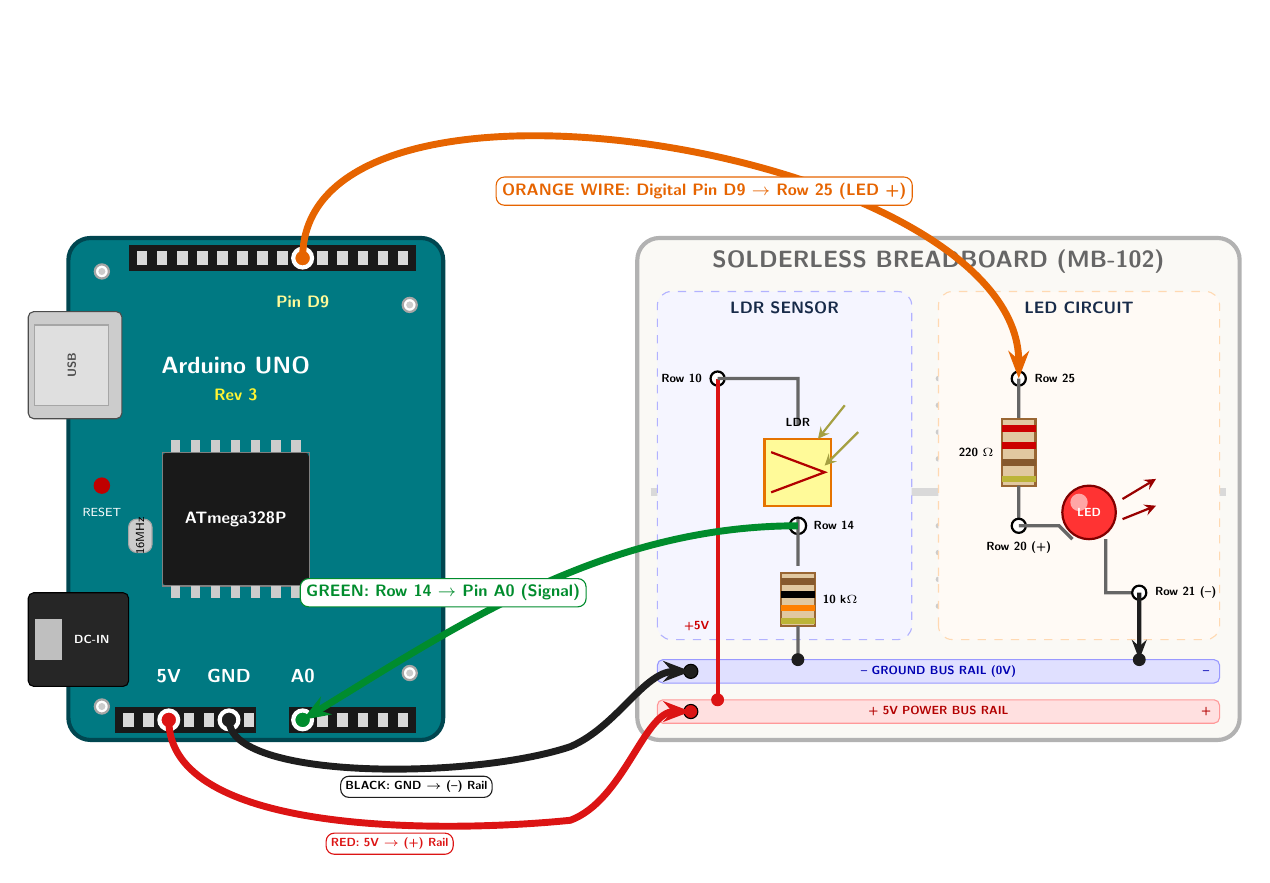
\begin{tikzpicture}[scale=0.85, every node/.style={transform shape}]

  % =========================================================================
  % ARDUINO UNO R3 (LEFT SIDE: X = 0 to 5.6, Y = 0.5 to 8.0)
  % =========================================================================
  % PCB Outline
  \fill[arduinoTeal!90!black, rounded corners=8pt] (0, 0.5) rectangle (5.6, 8.0);
  \draw[arduinoDark, line width=1.5pt, rounded corners=8pt] (0, 0.5) rectangle (5.6, 8.0);

  % Mounting holes
  \foreach \hx/\hy in {0.5/7.5, 0.5/1.0, 5.1/1.5, 5.1/7.0} {
    \filldraw[fill=white, draw=gray!70, thick] (\hx, \hy) circle (3pt);
    \fill[gray!40] (\hx, \hy) circle (1.5pt);
  }

  % USB Port (silver metal)
  \fill[gray!40, draw=black!70, rounded corners=2pt] (-0.6, 5.3) rectangle (0.8, 6.9);
  \draw[gray!70, fill=gray!25] (-0.5, 5.5) rectangle (0.6, 6.7);
  \node[font=\tiny\bfseries, text=black!70, rotate=90] at (0.05, 6.1) {USB};

  % DC Barrel Jack (black)
  \fill[black!85, draw=black, rounded corners=2pt] (-0.6, 1.3) rectangle (0.9, 2.7);
  \fill[gray!50] (-0.5, 1.7) rectangle (-0.1, 2.3);
  \node[font=\tiny\bfseries, text=white] at (0.35, 2.0) {DC-IN};

  % Reset Button (red)
  \fill[red!75!black, circle] (0.5, 4.3) circle (3.5pt);
  \node[font=\tiny, text=white] at (0.5, 3.9) {RESET};

  % Microcontroller ATmega328P DIP-28
  \fill[black!90, rounded corners=2pt] (1.4, 2.8) rectangle (3.6, 4.8);
  \draw[black!50, thin] (1.4, 2.8) rectangle (3.6, 4.8);
  \node[font=\scriptsize\bfseries, text=white] at (2.5, 3.8) {ATmega328P};
  % IC Pins
  \foreach \x in {1.6, 1.9, 2.2, 2.5, 2.8, 3.1, 3.4} {
    \fill[gray!40] (\x-0.07, 2.62) rectangle (\x+0.07, 2.8);
    \fill[gray!40] (\x-0.07, 4.8) rectangle (\x+0.07, 4.98);
  }

  % Crystal 16MHz
  \fill[gray!40, draw=gray!70, rounded corners=3pt] (0.9, 3.3) rectangle (1.25, 3.8);
  \node[font=\tiny, rotate=90] at (1.07, 3.55) {16MHz};

  % Board Title
  \node[font=\bfseries\normalsize, text=white] at (2.5, 6.1) {Arduino UNO};
  \node[font=\scriptsize\bfseries, text=yellow!80!white] at (2.5, 5.65) {Rev 3};

  % TOP HEADER (Digital I/O Pins)
  \fill[black!90] (0.9, 7.5) rectangle (5.2, 7.9);
  \foreach \x in {1.1, 1.4, 1.7, 2.0, 2.3, 2.6, 2.9, 3.2, 3.5, 3.8, 4.1, 4.4, 4.7, 5.0} {
    \fill[gray!30] (\x-0.08, 7.6) rectangle (\x+0.08, 7.8);
  }

  % D9 pin node on top header (x = 3.5)
  \coordinate (ardD9) at (3.5, 7.7);
  \filldraw[wireOrange, draw=white, line width=1.5pt] (ardD9) circle (4pt);
  \node[font=\scriptsize\bfseries, text=yellow!40!white, below=4pt] at (3.5, 7.4) {Pin D9};

  % BOTTOM HEADER - POWER
  \fill[black!90] (0.7, 0.6) rectangle (2.8, 1.0);
  \foreach \x in {0.9, 1.2, 1.5, 1.8, 2.1, 2.4, 2.7} {
    \fill[gray!30] (\x-0.08, 0.7) rectangle (\x+0.08, 0.9);
  }
  % 5V Pin (at x=1.5)
  \coordinate (ard5V) at (1.5, 0.8);
  \filldraw[wireRed, draw=white, line width=1.5pt] (ard5V) circle (4pt);
  \node[font=\footnotesize\bfseries, text=white, above=4pt] at (1.5, 1.1) {5V};

  % GND Pin (at x=2.4)
  \coordinate (ardGND) at (2.4, 0.8);
  \filldraw[wireBlack, draw=white, line width=1.5pt] (ardGND) circle (4pt);
  \node[font=\footnotesize\bfseries, text=white, above=4pt] at (2.4, 1.1) {GND};

  % BOTTOM HEADER - ANALOG IN
  \fill[black!90] (3.3, 0.6) rectangle (5.2, 1.0);
  \foreach \x in {3.5, 3.8, 4.1, 4.4, 4.7, 5.0} {
    \fill[gray!30] (\x-0.08, 0.7) rectangle (\x+0.08, 0.9);
  }
  % A0 Pin (at x=3.5)
  \coordinate (ardA0) at (3.5, 0.8);
  \filldraw[wireGreen, draw=white, line width=1.5pt] (ardA0) circle (4pt);
  \node[font=\footnotesize\bfseries, text=white, above=4pt] at (3.5, 1.1) {A0};

  % =========================================================================
  % SOLDERLESS BREADBOARD (RIGHT SIDE: X = 8.5 to 17.5, Y = 0.5 to 8.0)
  % =========================================================================
  \fill[breadboardBg, draw=gray!60, line width=1.5pt, rounded corners=8pt] (8.5, 0.5) rectangle (17.5, 8.0);
  \node[font=\normalsize\bfseries, text=gray!80!black] at (13.0, 7.65) {SOLDERLESS BREADBOARD (MB-102)};

  % Central Divider groove
  \draw[gray!30, line width=3pt] (8.7, 4.2) -- (17.3, 4.2);

  % Breadboard grid holes (visual cue)
  \foreach \gx in {9.1, 9.7, 10.3, 10.9, 11.5, 12.1, 13.0, 13.6, 14.2, 14.8, 15.4, 16.0, 16.6} {
    \foreach \gy in {2.5, 2.9, 3.3, 3.7, 4.7, 5.1, 5.5, 5.9} {
      \fill[gray!40] (\gx, \gy) circle (1.2pt);
    }
  }

  % Bottom Power Rails: Blue (GND) at y=1.5, Red (+5V) at y=0.9
  \fill[blue!12, draw=blue!40, rounded corners=2pt] (8.8, 1.35) rectangle (17.2, 1.7);
  \node[font=\tiny\bfseries, text=blue!70!black] at (9.0, 1.525) {--};
  \node[font=\tiny\bfseries, text=blue!70!black] at (13.0, 1.525) {-- GROUND BUS RAIL (0V)};
  \node[font=\tiny\bfseries, text=blue!70!black] at (17.0, 1.525) {--};
  \coordinate (bbGNDRail) at (9.3, 1.525);
  \filldraw[wireBlack, draw=black] (bbGNDRail) circle (3pt);

  % Red (+5V) Rail
  \fill[red!12, draw=red!40, rounded corners=2pt] (8.8, 0.75) rectangle (17.2, 1.1);
  \node[font=\tiny\bfseries, text=red!70!black] at (9.0, 0.925) {+};
  \node[font=\tiny\bfseries, text=red!70!black] at (13.0, 0.925) {+ 5V POWER BUS RAIL};
  \node[font=\tiny\bfseries, text=red!70!black] at (17.0, 0.925) {+};
  \coordinate (bbRedRail) at (9.3, 0.925);
  \filldraw[wireRed, draw=black] (bbRedRail) circle (3pt);

  % --- SUB-CIRCUIT 1: LDR SENSOR DIVIDER (Left side of breadboard) ---
  \draw[rounded corners=5pt, fill=blue!4, draw=blue!30, dashed] (8.8, 2.0) rectangle (12.6, 7.2);
  \node[font=\scriptsize\bfseries\color{primaryDark}] at (10.7, 6.95) {LDR SENSOR};

  % Row 10 (Tie Point)
  \coordinate (row10) at (9.7, 5.9);
  \filldraw[fill=white, draw=black, thick] (row10) circle (3pt) node[left=3pt, font=\tiny\bfseries] {Row 10};

  % Internal Jumper: +5V Rail to Row 10
  \draw[line width=1.5pt, wireRed] (9.7, 1.1) -- (9.7, 5.9);
  \filldraw[wireRed] (9.7, 1.1) circle (2.5pt);
  \node[font=\tiny\bfseries, text=red!80!black, left] at (9.7, 2.2) {+5V};

  % Row 14 (Divider Node)
  \coordinate (row14) at (10.9, 3.7);
  \filldraw[fill=white, draw=black, thick] (row14) circle (3.5pt) node[right=3pt, font=\tiny\bfseries] {Row 14};

  % LDR Component between Row 10 and Row 14
  \draw[line width=1.2pt, gray!80!black] (row10) -- (10.9, 5.9) -- (10.9, 5.2);
  \draw[line width=1.2pt, gray!80!black] (10.9, 3.8) -- (row14);
  \filldraw[fill=yellow!40, draw=orange!90!black, thick] (10.4, 4.0) rectangle (11.4, 5.0);
  \draw[thick, red!70!black] (10.5, 4.2) -- (11.3, 4.5) -- (10.5, 4.8);
  \node[font=\tiny\bfseries, text=black] at (10.9, 5.25) {LDR};
  % Light arrows
  \draw[->, >=stealth, thick, yellow!60!black] (11.6, 5.5) -- (11.2, 5.0);
  \draw[->, >=stealth, thick, yellow!60!black] (11.8, 5.1) -- (11.3, 4.6);

  % 10k Resistor from Row 14 to GND Rail
  \coordinate (res10kBottom) at (10.9, 1.7);
  \draw[line width=1.2pt, gray!80!black] (row14) -- (10.9, 3.1);
  \filldraw[fill=resistorBody, draw=brown!80!black, thick] (10.65, 2.2) rectangle (11.15, 3.0);
  % Color bands: Brown, Black, Orange, Gold
  \fill[brown!70!black] (10.65, 2.82) rectangle (11.15, 2.92);
  \fill[black] (10.65, 2.62) rectangle (11.15, 2.72);
  \fill[orange] (10.65, 2.42) rectangle (11.15, 2.52);
  \fill[yellow!70!black] (10.65, 2.24) rectangle (11.15, 2.32);
  \node[font=\tiny\bfseries, text=black, right] at (11.15, 2.6) {10 k$\Omega$};
  \draw[line width=1.2pt, gray!80!black] (10.9, 2.2) -- (res10kBottom);
  \filldraw[wireBlack] (res10kBottom) circle (2.5pt);

  % --- SUB-CIRCUIT 2: LED ACTUATOR DRIVE (Right side of breadboard) ---
  \draw[rounded corners=5pt, fill=orange!4, draw=orange!30, dashed] (13.0, 2.0) rectangle (17.2, 7.2);
  \node[font=\scriptsize\bfseries\color{primaryDark}] at (15.1, 6.95) {LED CIRCUIT};

  % Row 25 (Input from Pin D9)
  \coordinate (row25) at (14.2, 5.9);
  \filldraw[fill=white, draw=black, thick] (row25) circle (3pt) node[right=3pt, font=\tiny\bfseries] {Row 25};

  % 220 Ohm Resistor between Row 25 and Row 20
  \coordinate (row20) at (14.2, 3.7);
  \draw[line width=1.2pt, gray!80!black] (row25) -- (14.2, 5.3);
  \filldraw[fill=resistorBody, draw=brown!80!black, thick] (13.95, 4.3) rectangle (14.45, 5.3);
  % Color bands: Red, Red, Brown, Gold
  \fill[red!80!black] (13.95, 5.1) rectangle (14.45, 5.2);
  \fill[red!80!black] (13.95, 4.85) rectangle (14.45, 4.95);
  \fill[brown!70!black] (13.95, 4.6) rectangle (14.45, 4.7);
  \fill[yellow!70!black] (13.95, 4.35) rectangle (14.45, 4.45);
  \node[font=\tiny\bfseries, text=black, left] at (13.95, 4.8) {220 $\Omega$};
  \draw[line width=1.2pt, gray!80!black] (14.2, 4.3) -- (row20);

  % Row 20 (LED Anode)
  \filldraw[fill=white, draw=black, thick] (row20) circle (3pt) node[below=3pt, font=\tiny\bfseries] {Row 20 (+)};

  % LED between Row 20 and Row 21
  \coordinate (row21) at (16.0, 2.7);
  \draw[line width=1.2pt, gray!80!black] (row20) -- (14.8, 3.7) -- (15.0, 3.5);
  \draw[line width=1.2pt, gray!80!black] (row21) -- (15.5, 2.7) -- (15.5, 3.5);
  \filldraw[fill=red!80, draw=red!50!black, thick] (15.25, 3.9) circle (0.4cm);
  \fill[red!35] (15.1, 4.05) circle (0.13cm);
  \node[font=\tiny\bfseries, text=white] at (15.25, 3.9) {LED};
  % Light rays
  \draw[->, >=stealth, thick, red!60!black] (15.75, 4.1) -- (16.25, 4.4);
  \draw[->, >=stealth, thick, red!60!black] (15.75, 3.8) -- (16.25, 4.0);

  % Row 21 (LED Cathode)
  \filldraw[fill=white, draw=black, thick] (row21) circle (3pt) node[right=3pt, font=\tiny\bfseries] {Row 21 (--)};

  % Jumper from Row 21 (Cathode) to Bottom GND Rail
  \draw[wireBlack, line width=1.5pt, -{Stealth[length=2.5mm]}] (row21) -- (16.0, 1.7);
  \filldraw[wireBlack] (16.0, 1.7) circle (2.5pt);

  % =========================================================================
  % MAIN 4 JUMPER WIRES (INTERCONNECTS) - STRICTLY NON-CROSSING
  % =========================================================================

  % 1. ORANGE WIRE: Arduino D9 -> Row 25 (Upper Arc)
  \draw[line width=2.5pt, wireOrange, -{Stealth[length=3.5mm]}] 
       (ardD9) to[out=90, in=90, looseness=0.8] (row25);
  \node[fill=white, draw=wireOrange, rounded corners=3pt, inner sep=2.5pt, font=\scriptsize\bfseries, text=wireOrange] 
       at (9.5, 8.7) {ORANGE WIRE: Digital Pin D9 $\to$ Row 25 (LED +)};

  % 2. GREEN WIRE: Row 14 -> Arduino A0 (Middle Arc)
  \draw[line width=2.5pt, wireGreen, -{Stealth[length=3.5mm]}] 
       (row14) .. controls (8.0, 3.7) and (5.8, 2.2) .. (ardA0);
  \node[fill=white, draw=wireGreen, rounded corners=3pt, inner sep=2.5pt, font=\scriptsize\bfseries, text=wireGreen] 
       at (5.6, 2.7) {GREEN: Row 14 $\to$ Pin A0 (Signal)};

  % 3. BLACK WIRE: Arduino GND -> Breadboard Blue Rail (Inner Lower Curve)
  \draw[line width=2.5pt, wireBlack, -{Stealth[length=3.5mm]}] 
       (ardGND) .. controls (2.4, -0.1) and (6.0, -0.1) .. (7.5, 0.4) .. controls (8.2, 0.7) and (8.6, 1.525) .. (bbGNDRail);
  \node[fill=white, draw=wireBlack, rounded corners=3pt, inner sep=2pt, font=\tiny\bfseries, text=black] 
       at (5.2, -0.2) {BLACK: GND $\to$ (--) Rail};

  % 4. RED WIRE: Arduino 5V -> Breadboard Red Rail (Outer Lower Curve)
  \draw[line width=2.5pt, wireRed, -{Stealth[length=3.5mm]}] 
       (ard5V) .. controls (1.5, -0.9) and (5.5, -0.9) .. (7.5, -0.7) .. controls (8.3, -0.4) and (8.6, 0.925) .. (bbRedRail);
  \node[fill=white, draw=wireRed, rounded corners=3pt, inner sep=2pt, font=\tiny\bfseries, text=wireRed] 
       at (4.8, -1.05) {RED: 5V $\to$ (+) Rail};

\end{tikzpicture}
\end{center}

\vspace{-0.2cm}
\begin{center}
{\small\textbf{Figure 1: Graphical Wire Connection Diagram showing Arduino UNO R3 Header-to-Breadboard Connections.}}
\end{center}

\begin{center}
\footnotesize
\renewcommand{\arraystretch}{1.12}
\begin{tabularx}{\textwidth}{|l|>{\raggedright\arraybackslash}p{3.2cm}|>{\raggedright\arraybackslash}p{3.6cm}|X|}
\hline
\textbf{Wire Color} & \textbf{Origin Pin (Arduino)} & \textbf{Destination Point (Breadboard)} & \textbf{Circuit Function / Signal} \\
\hline
\textcolor{wireOrange}{\textbf{Orange}} & Pin D9 (Digital PWM Header) & Row 25 (Top Lead of 220\,$\Omega$ Resistor) & Switched Output Gate Drive (+5V Active) \\
\hline
\textcolor{wireGreen}{\textbf{Green}} & Pin A0 (Analog In Header) & Row 14 (Divider Tap Junction Node) & Analog Light Sensor Voltage Signal \\
\hline
\textbf{Black} & Pin GND (Power Header) & Blue Bus Rail (--) (Lower Ground Rail) & 0V System Common Ground Return \\
\hline
\textcolor{wireRed}{\textbf{Red}} & Pin 5V (Power Header) & Red Bus Rail (+) (Lower Power Rail) & +5V Regulated DC Supply Rail \\
\hline
\end{tabularx}
\vspace{0.15cm}
{\footnotesize\textbf{Table 2: Wire Connection Quick-Reference Matrix.}}
\end{center}

\newpage

% ==============================================================================
% PHASE 3: BREADBOARD WIRING SEQUENCE
% ==============================================================================
\section*{Phase 3: Breadboard Step-by-Step Wiring Sequence}

\begin{notebox}{Important Safety Rule}
Keep the Arduino UNO \textbf{completely disconnected from USB power} while inserting components and jumper wires on the breadboard to prevent accidental shorts.
\end{notebox}

\begin{stepbox}{Step 2.1: Establish Main Power Rails}
\begin{enumerate}
    \item Take a \textbf{Red jumper wire}: Connect Arduino header pin \textbf{5V} to the \textbf{Red (+) power rail} on the breadboard.
    \item Take a \textbf{Black jumper wire}: Connect Arduino header pin \textbf{GND} to the \textbf{Blue (--) ground rail} on the breadboard.
\end{enumerate}
\end{stepbox}

\begin{stepbox}{Step 2.2: Assemble the LDR Potential Divider (Sensor Subcircuit)}
\begin{enumerate}
    \item Insert the two legs of the \textbf{LDR (GL5528)} into \textbf{Row 10} and \textbf{Row 14} on the breadboard.
    \item Connect a short jumper wire from \textbf{Row 10} (LDR Leg 1) to the \textbf{Red (+) 5V power rail}.
    \item Insert one leg of the \textbf{10 k$\Omega$ resistor} (\texttt{CFR-25JR-10K}) into \textbf{Row 14} (shared with LDR Leg 2).
    \item Insert the second leg of the \textbf{10 k$\Omega$ resistor} into the \textbf{Blue (--) Ground rail}.
    \item Take a \textbf{Green jumper wire}: Connect from \textbf{Row 14} (the shared divider tap junction) to Arduino Analog Pin \textbf{A0}.
\end{enumerate}
\end{stepbox}

\begin{stepbox}{Step 2.3: Assemble the LED Luminaire (Actuator Subcircuit)}
\begin{enumerate}
    \item Insert the \textbf{5mm LED} (\texttt{WP7113ID}):
    \begin{itemize}
        \item Insert the \textbf{Longer Lead (Anode +)} into \textbf{Row 20}.
        \item Insert the \textbf{Shorter Lead (Cathode --)} into \textbf{Row 21}.
    \end{itemize}
    \item Insert the \textbf{220 $\Omega$ resistor} (\texttt{CFR-25JR-220R}) between \textbf{Row 20} (with LED Anode) and \textbf{Row 25}.
    \item Take an \textbf{Orange jumper wire}: Connect from \textbf{Row 25} (the other side of the $220\,\Omega$ resistor) to Arduino Digital Pin \textbf{D9}.
    \item Take a \textbf{Black jumper wire}: Connect from \textbf{Row 21} (LED Cathode) to the \textbf{Blue (--) Ground rail}.
\end{enumerate}
\end{stepbox}

\begin{stepbox}{Step 2.4: Pre-Power Visual Checklist}
\begin{itemize}
    \item[$\square$] LDR is connected between $+5\,\text{V}$ rail and Row 14.
    \item[$\square$] $10\,\text{k}\Omega$ resistor connects Row 14 to GND rail.
    \item[$\square$] Green wire connects Row 14 to Analog Pin A0.
    \item[$\square$] Orange wire connects Digital Pin D9 to the $220\,\Omega$ resistor.
    \item[$\square$] LED Anode (long leg) connects to the $220\,\Omega$ resistor; Cathode (short leg) connects to GND.
\end{itemize}
\end{stepbox}

\newpage

% ==============================================================================
% PHASE 4 & PHASE 5: FIRMWARE FLASHING & INTERACTIVE TESTING
% ==============================================================================
\section*{Phase 4: Firmware Flashing in Arduino IDE}

\begin{stepbox}{Step 3.1: Connect Arduino to Workstation}
Plug the USB Type-A to Type-B cable into the Arduino UNO and your computer's USB port. The green `ON` LED on the Arduino board will illuminate steadily.
\end{stepbox}

\begin{stepbox}{Step 3.2: Configure Board and Port in Arduino IDE}
\begin{enumerate}
    \item Open the \textbf{Arduino IDE}.
    \item Go to: \textbf{Tools $\to$ Board $\to$ Arduino AVR Boards $\to$ Arduino Uno}.
    \item Go to: \textbf{Tools $\to$ Port} and select the active COM port assigned to the board (e.g., \texttt{COM3}, \texttt{COM4} --- marked as \emph{"Arduino Uno"}).
\end{enumerate}
\end{stepbox}

\begin{stepbox}{Step 3.3: Load and Upload Sketch}
\begin{enumerate}
    \item Open the project sketch: \texttt{Automatic\_Night\_Light.ino}.
    \item Click the \textbf{Verify} button (checkmark icon) to compile. Check that there are zero compiler errors.
    \item Click the \textbf{Upload} button (right-arrow icon). The `TX` and `RX` yellow LEDs will flash rapidly for 2 seconds until the IDE displays: \textbf{"Done uploading"}.
\end{enumerate}
\end{stepbox}

\vspace{0.2cm}

\section*{Phase 5: Live Calibration \& Functional Testing}

\begin{stepbox}{Step 4.1: Open Serial Monitor Telemetry}
\begin{enumerate}
    \item Click the magnifying glass icon at the top right corner of the IDE to launch the \textbf{Serial Monitor}.
    \item Set the Baud rate dropdown at the bottom right corner to \textbf{9600 baud}.
    \item Verify the live telemetry stream:
    \begin{center}
    \texttt{ADC: 839 | V: 4.10V | Luminaire: INACTIVE (OFF)}
    \end{center}
\end{enumerate}
\end{stepbox}

\begin{stepbox}{Step 4.2: Normal Room Light Baseline Test}
Under standard room or lab lighting:
\begin{itemize}
    \item Verify that the ADC value is between \textbf{600 and 850} ($V_{\text{out}} \approx 3.0\,\text{V} - 4.2\,\text{V}$).
    \item Confirm that the LED remains completely \textbf{OFF} (Daylight detected).
\end{itemize}
\end{stepbox}

\begin{stepbox}{Step 4.3: Nightfall Simulation (Darkness Test)}
Cover the LDR completely using your finger or an opaque object (e.g., black paper or notebook):
\begin{itemize}
    \item Observe the Serial Monitor: the ADC value drops sharply below \textbf{400} ($V_{\text{out}} < 1.95\,\text{V}$).
    \item Confirm: The LED turns \textbf{ON automatically and brightly}!
    \item The Serial Monitor reports: \texttt{Luminaire: ACTIVE (ON) [Nightfall Detected]}.
\end{itemize}
\end{stepbox}

\newpage

% ==============================================================================
% PHASE 5 (CONT.) & PHASE 6: HYSTERESIS, TROUBLESHOOTING & EVALUATION
% ==============================================================================
\begin{stepbox}{Step 4.4: Hysteresis Deadband Verification (Anti-Flicker Demo)}
Gradually pull your finger away from the LDR:
\begin{itemize}
    \item Notice that when the ADC value climbs through the twilight transition region between \textbf{400 and 500}, the LED \textbf{remains solidly ON}. It does \textbf{NOT} flicker!
    \item Only when the light level rises fully above \textbf{500} ($V_{\text{out}} \ge 2.44\,\text{V}$) does the LED turn OFF.
    \item This proves that the \textbf{100-count Schmitt trigger deadband} successfully prevents flickering at dusk!
\end{itemize}
\end{stepbox}

\vspace{0.1cm}

\section*{Phase 6: Troubleshooting Reference Table}

\begin{center}
\small
\renewcommand{\arraystretch}{1.2}
\begin{tabularx}{\textwidth}{|>{\raggedright\arraybackslash}p{4.0cm}|>{\raggedright\arraybackslash}p{4.2cm}|X|}
\hline
\textbf{Observed Issue} & \textbf{Probable Cause} & \textbf{Step-by-Step Fix} \\
\hline
LED never turns ON, even when LDR is covered. & 
1. LED inserted backwards. \newline
2. Loose jumper wire in D9. \newline
3. Burned-out LED. & 
Reverse LED leads (long lead connects to D9 via $220\,\Omega$). Verify wire is in Pin D9. Swap with another LED. \\
\hline
LED stays ON all the time, even in daylight. & 
1. $10\,\text{k}\Omega$ resistor loose. \newline
2. LDR not receiving $+5\,\text{V}$. \newline
3. Pin A0 floating. & 
Ensure $10\,\text{k}\Omega$ resistor connects from node A0 to GND rail. Confirm LDR high side is in $+5\,\text{V}$. \\
\hline
ADC readings jump wildly or erratically. & 
1. 50/60\,Hz AC line noise. \newline
2. Loose breadboard ties. & 
Firmware already includes a 10-sample moving average filter. Press wires firmly into breadboard tie holes. \\
\hline
Serial Monitor displays gibberish / strange characters. & 
Baud rate mismatch. & 
Change the baud rate dropdown at the bottom right of the Serial Monitor to \textbf{9600 baud}. \\
\hline
\end{tabularx}
\vspace{0.15cm}
{\small\textbf{Table 3: Common Fault Identification \& Corrective Actions Matrix.}}
\end{center}

\vspace{0.2cm}

\begin{stepbox}{Laboratory Performance Evaluation \& Sign-Off}
\begin{tabularx}{\textwidth}{X X X}
\textbf{Student Name:} \hrulefill & \textbf{Roll Number:} \hrulefill & \textbf{Date:} \hrulefill \\[0.25cm]
\textbf{Circuit Assembly (4M):} \hrulefill & \textbf{Firmware \& Calibration (4M):} \hrulefill & \textbf{Viva-Voce (2M):} \hrulefill \\[0.25cm]
\multicolumn{2}{l}{\textbf{Faculty Evaluator Signature:} \hrulefill} & \textbf{Total Marks:} \quad \textbf{/ 10} \\
\end{tabularx}
\end{stepbox}

\end{document}
